\section{恒定磁场的高斯定理与安培环路定理}

\subsection{恒定磁场的高斯定理}

1.\textbf{通过任意闭合曲面的磁通量总等于零。}
即$$\oint_{S}\mathbf{B}\mathrm{d}S=0$$

2.激发静电场的场源（电荷）是电场线的源头或尾闾，所以静电场是属于发散状的场，可称作有源场；而磁场的磁感应线无头无尾，永远是闭合的，所以磁场可称作无源场。

3.磁场的高斯定理与静电场的高斯定理不对称的根本原因是自然界不存在单
个磁极（即磁单极子）。

\subsection{恒定磁场的安培环路定理}

1.\textbf{在恒定磁场中，磁感应强度治任一闭合路径的线积分等于$\mu_{0}$倍的穿过以闭合曲线为边界的任意曲面的各恒定电流的代数和,也称为矢量的环流}
即$$\oint\mathbf{B}\mathrm{d}\mathbf{l}=\mu_{0}\sum I_{i}$$

2.通常把磁场叫做有旋场，而$\mathbf{E}$的环流恒等于零，所以把静电场叫做无旋场。

3.讨论:

(1)B是空间全部电流产生的磁场。

(2)对任意形式的恒定电流所激发的磁场都成立，对任何形形状的闭合路径都成立。

\subsection{典型安培环路定理的应用}

\subsubsection{无限长直电流的磁场}

\begin{figure}[h]
	\centering
	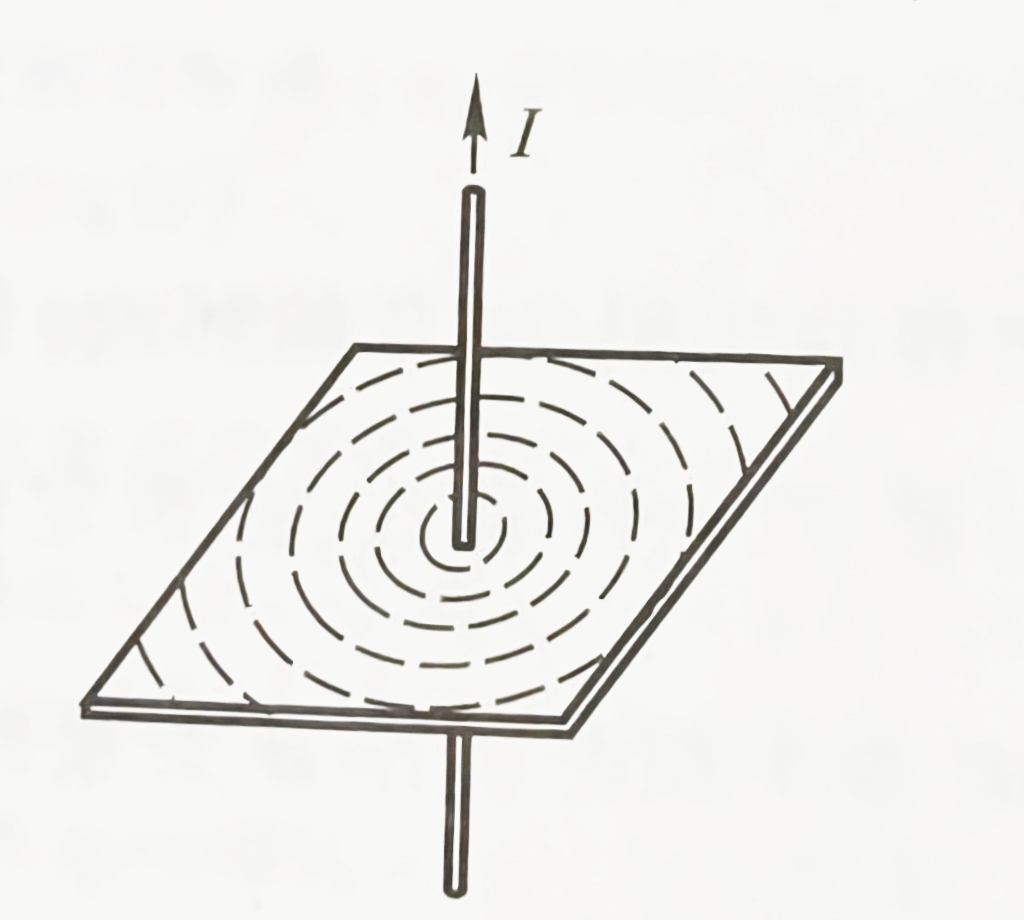
\includegraphics[width=0.4\linewidth]{images/无限长直导线的磁场}
	\caption{无限长直导线的磁场}
	\label{fig:}
\end{figure}

磁场为一圈一圈的同心圆，取闭合路径为磁场的同心圆，半径为r。

由安培环路定理$$ \oint\mathbf{B}\mathrm{d}\mathbf{l}=\oint B\mathrm{d}l=B\oint\mathrm{d}l=\mu_{0}\sum I_{i}$$

则$$2B\pi r=\mu_{0}I$$
$$B=\frac{\mu_{0}I}{2\pi r}$$

方向与电流流向呈右手螺旋定则

\subsubsection{长直圆柱形载流导线内外的磁场}

\begin{figure}[h]
	\centering
	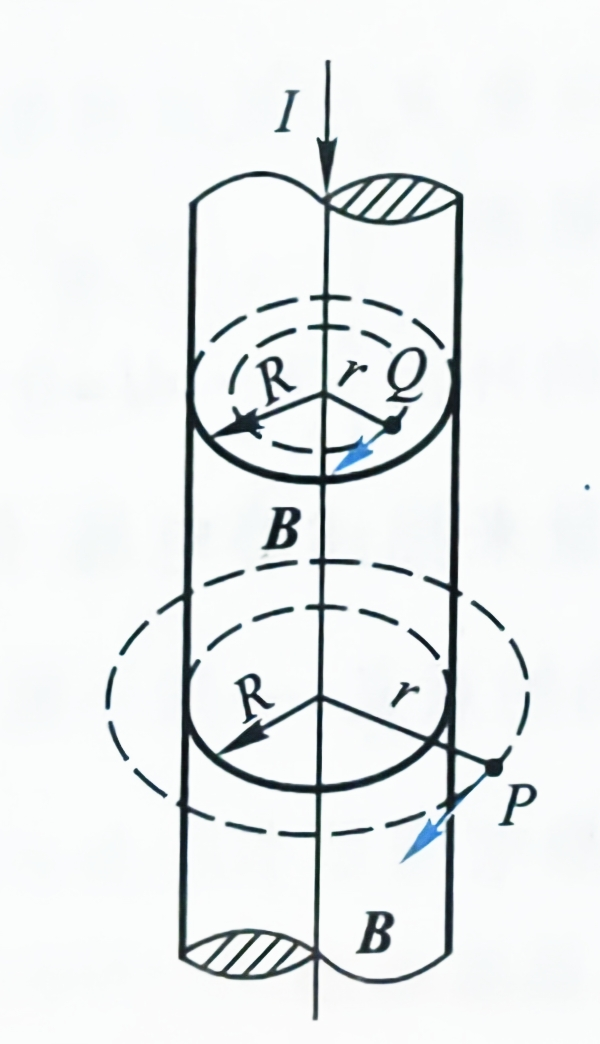
\includegraphics[width=0.2\linewidth]{images/长直圆柱形载流导线内外的磁场}
	\caption{长直圆柱形载流导线内外的磁场}
	\label{fig:}
\end{figure}

从轴线方向看，上下左右对称的电流对圆柱形载流导线外一点的磁感应强度是对称的，因此磁场呈轴对称分布，磁感应线为垂直于轴线的同心圆。

圆柱的半径为R，取半径为r的同心圆为闭合路径。

则由安培环路定理$$\oint\mathbf{B}\mathrm{d}\mathbf{l}=\oint B\mathrm{d}l=B\oint\mathrm{d}l=\mu_{0}\sum I_{i} $$

1.当r>R时，则$$2B\pi r=\mu_{0}I$$

2.当r<R时，则$$2B\pi r=\mu_{0}\frac{\pi r^{2}}{\pi R_{^{2}}}$$

则$$\left\{
\begin{aligned}
	B&=\frac{\mu_{0}I}{2\pi r}，,r>R\\
	B&=\frac{\mu_{0}Ir}{2\pi R}，,r<R
\end{aligned}
\right.$$

\subsubsection{均匀密绕无限长直螺线管的磁场}

\begin{figure}[h]
	\centering
	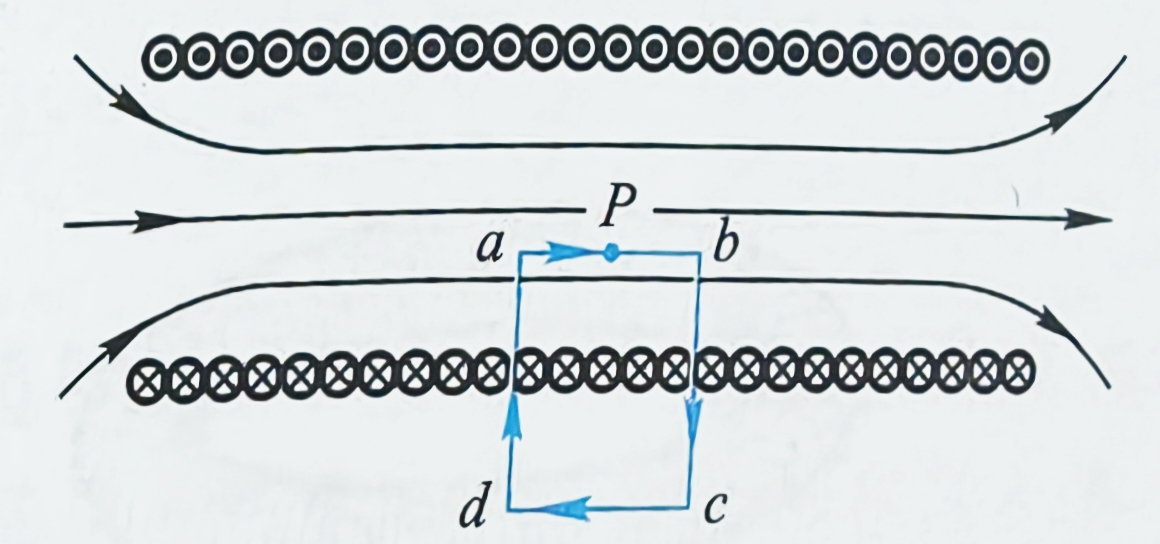
\includegraphics[width=0.5\linewidth]{images/均匀密绕无限长直螺线管的磁场}
	\caption{均匀密绕无限长直螺线管的磁场}
	\label{fig:}
\end{figure}

已知有N匝线圈，电流为I，数密度为n。

P为螺线管内一点，由分析可知，P点磁感线的方向为过点P且平行于轴线的方向，该同一直线上其他点方向也沿该直线。即\textbf{P点所在的平行直线上大小相同，方向相同}

取闭合回路为矩形abcda

则由安培环路定理$$\oint\mathbf{B}\mathrm{d}\mathbf{l}=Bl_{ab}=\mu_{0}nl_{ab}I$$

则$$B=\mu_{0}nI $$

在螺线管外部，磁感线相互抵消，磁感应强度很小，$B_{内}\gg B_{外}$，可视做$B_{外}=0 $，所以多匝线圈一般被视为储能原件。

\subsubsection{均匀载流螺绕环的磁场}

\begin{figure}[h]
	\centering
	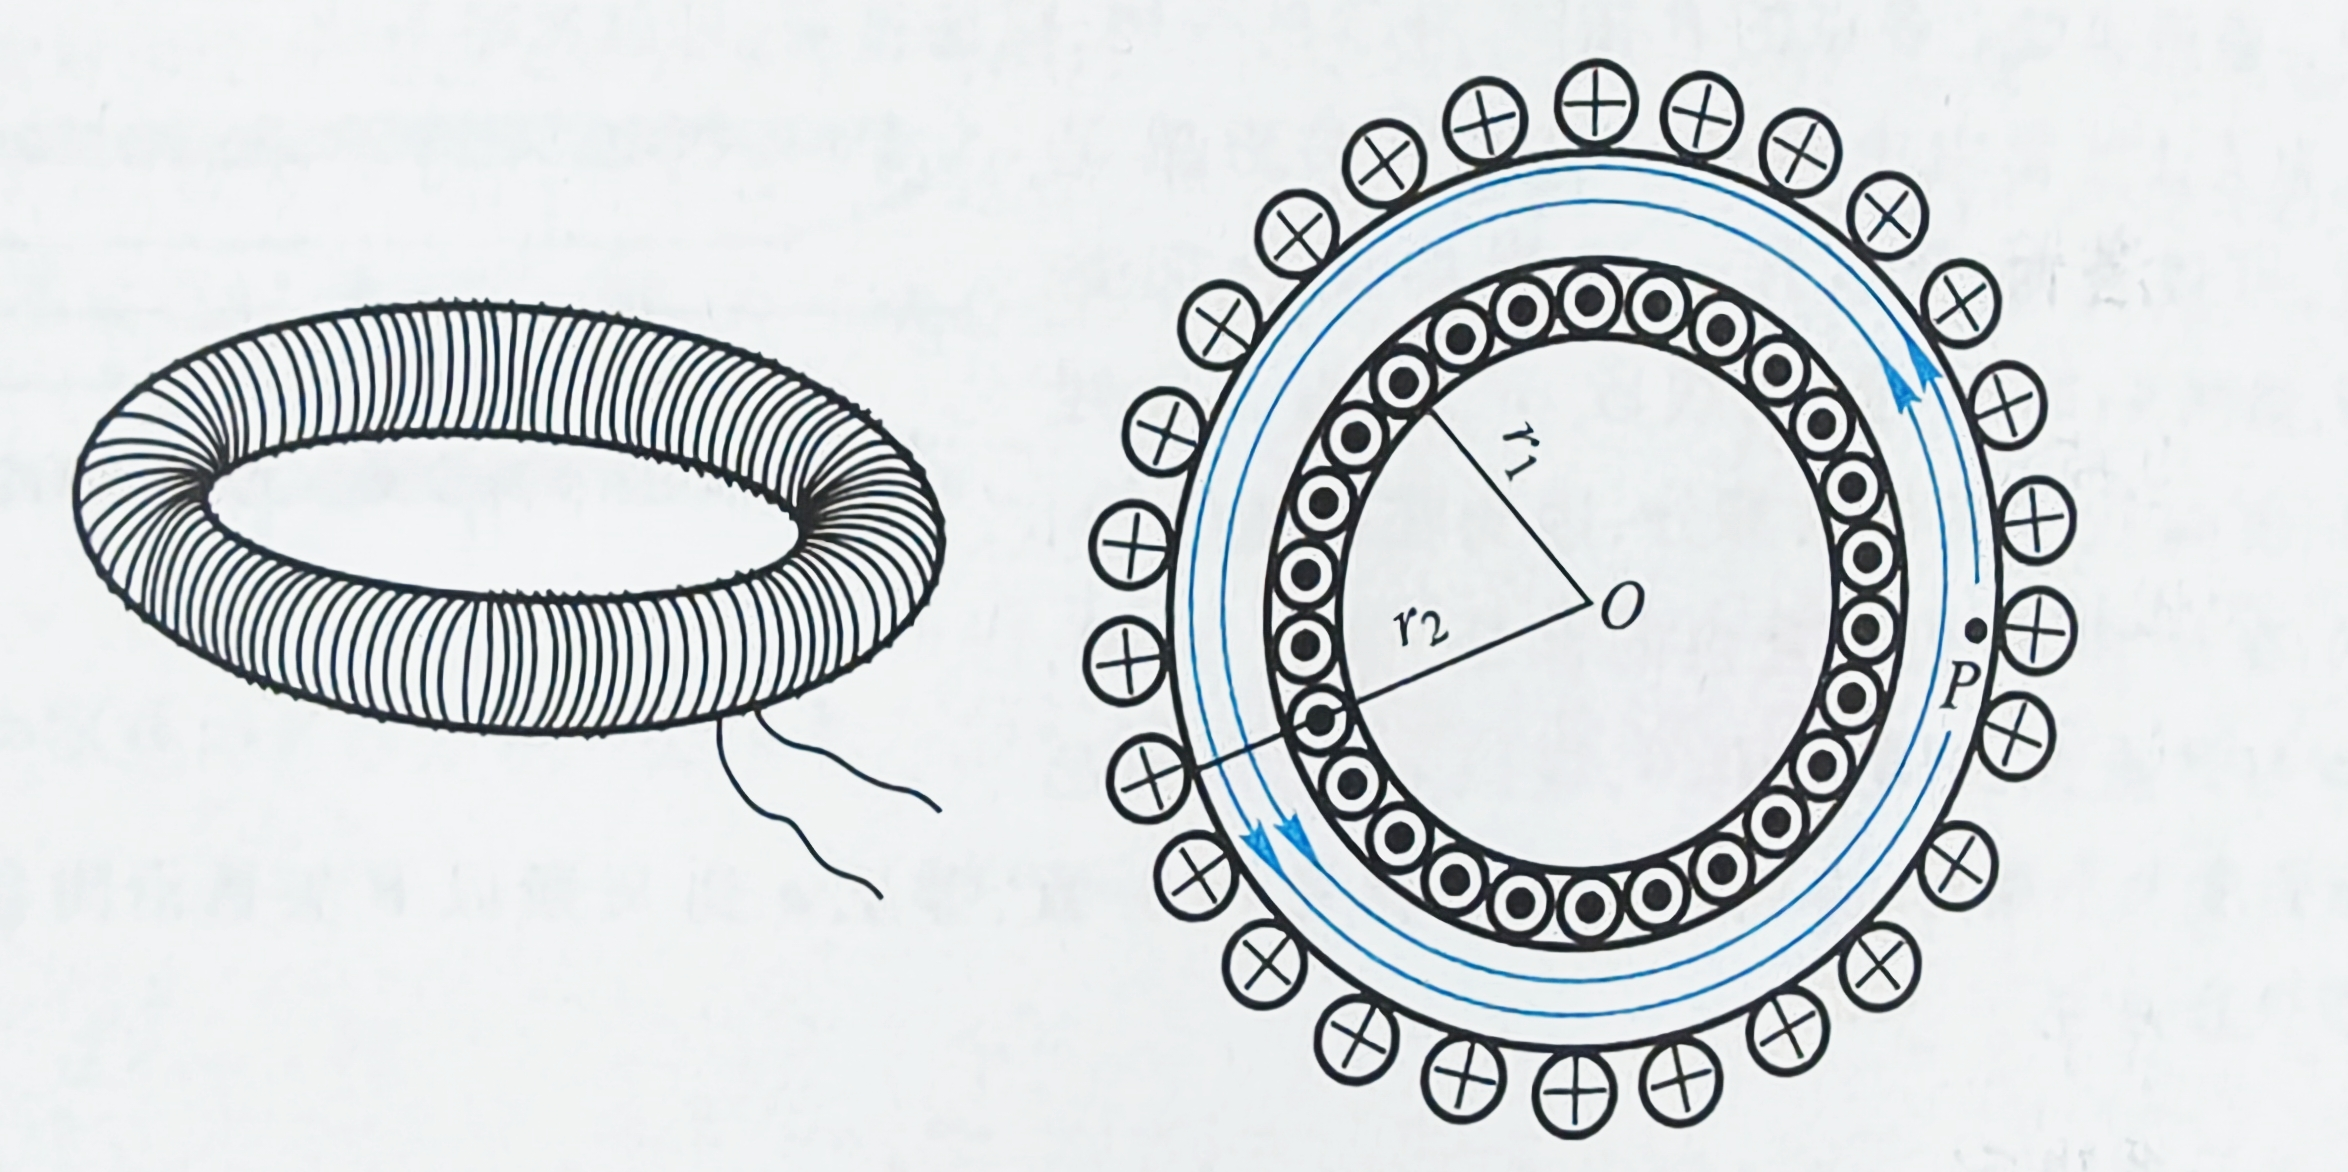
\includegraphics[width=0.6\linewidth]{images/均匀载流螺绕环的磁场}
	\caption{}
	\label{fig:}
\end{figure}

已知内径为$R_{1}$，外径为$R_{2}$，电流为I，匝数为N。

经放大图分析，螺绕环的磁感线为其内部的同心圆，取半径为r的同心圆为闭合路径。

则由安培环路定理$$\oint\mathbf{B}\mathrm{d}\mathbf{l}=\oint B\mathrm{d}l=B\oint\mathrm{d}l=\mu_{0}\sum I_{i} $$

1.当$R_{1}$<r<$R_{2}$时，则$$2B\pi r=\mu_{0}NI$$

2.当r>$R_{2}$时，电流相互抵消，则$$2B\pi r=0$$

则$$\left\{
\begin{aligned}
	B&=\frac{\mu_{0}NI}{2\pi r},R_{1}<r<R_{2}\\
	B&=0,r>R_{2}
\end{aligned}
\right.$$